\chapter{Tensor Parallelism}

\section{Introduction}

\begin{figure}[t]
	\centering
	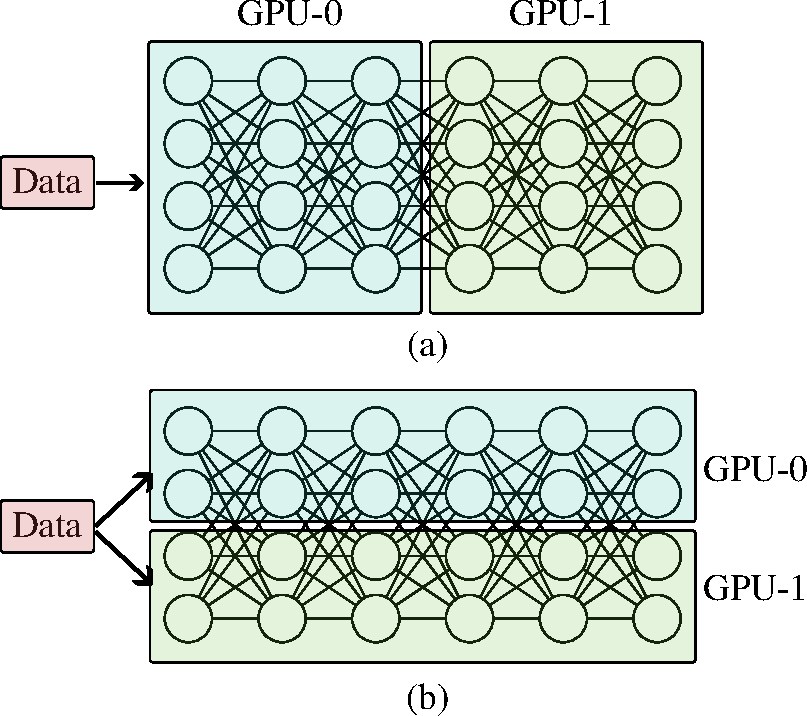
\includegraphics[scale=0.8]{./images/tensor_parallel.pdf}
	\caption{(a): Pipeline parallelism. (b) Tensor parallelism.}
\end{figure}

Let's go over an example:
\begin{itemize}
	\item \( x \) is a row vector of shape \([1, d_\text{in}]\) (the input).  
	\item \( W \) is a weight matrix of shape \([d_\text{in}, d_\text{out}]\).  
	\item \(\text{output}\) is \([1, d_\text{out}]\).
\end{itemize}

We have two GPUs, GPU 0 and GPU 1. We want to split (shard) the weight matrix \( W \) across two GPUs. One common approach is column parallelism:  
\begin{itemize}
	\item GPU 0 holds columns \([0,1]\)  
	\item GPU 1 holds columns \([2,3]\)  
\end{itemize}

This means each GPU stores some columns of \(W\). Let's denote:

\[
W = \bigl[W_{\text{left}} \,\big|\ W_{\text{right}}\bigr]
\]

where
\begin{itemize}
	\item \( W_{\text{left}} \) is a \(4 \times 2\) matrix on GPU 0,  
	\item \( W_{\text{right}} \) is a \(4 \times 2\) matrix on GPU 1.
\end{itemize}

In numeric form, suppose
\[
W =
\begin{bmatrix}
1 & 2 & 5 & 6\\
3 & 4 & 7 & 8\\
2 & 0 & 3 & 1\\
-1 & 4 & 8 & 2
\end{bmatrix}.
\]

Then, for column parallel:
\begin{itemize}
	\item GPU 0:  
  \[
  W_{\text{left}} = 
  \begin{bmatrix}
  1 & 2 \\
  3 & 4 \\
  2 & 0 \\
  -1 & 4 
  \end{bmatrix}.
  \]
\item GPU 1:  
  \[
  W_{\text{right}} = 
  \begin{bmatrix}
  5 & 6 \\
  7 & 8 \\
  3 & 1 \\
  8 & 2
  \end{bmatrix}.
  \]
\end{itemize}

Given the input
\[
x = [\, 1,\ 2,\ 0,\ 1\,].
\]

We can treat \(x\) as a row vector \([1,4]\). For column parallelism, each GPU needs the entire input \(x\) so it can multiply by its subset of columns:
\begin{itemize}
	\item We copy the \( x \) to both GPU 0 and GPU 1.  
		\begin{itemize}
			\item This is typically a small overhead compared to storing large weight matrices.
		\end{itemize}
	\item Then, compute the matrix multiplications for each matrix.
	\item Finally, concatenate the outputs.
\end{itemize}

\[
\text{output} = [\, \text{partial}_0 \;\big|\; \text{partial}_1\,] = [\,6,\ 14,\ 27,\ 24\,].
\]
\begin{itemize}
	\item Some frameworks do a ring-all-gather, or they might place this final output on one GPU if needed, etc. 
\end{itemize}

When we do backprop, we can update the model's parameters in the opposite direction. 

